\section{Quantitative excitation bounds}\label{sec:05}
The all-mode estimates have computable constants. Table~\ref{tab:numeric} separates the directly integrated modes from the analytic tails. For orders one and two the lowest mixed $k=2,M=1$ block alone has probabilities $7.8066279\ldots\times10^{-7}$ and $1.0775406\ldots\times10^{-8}$ per copy. Thus both finite energies or counts asserted positive receive a nonzero contribution before any extrapolation. The round solution has zero mixing for every mode since its Pauli axis is constant in time.
\begin{table}[ht]\centering\small
\begin{tabular}{llll}\toprule
Quantity & $k\le24$ enclosure & $k>24$ upper bound & All modes\\\midrule
$10^{5}S_1$ & $[6.11898256,6.11898265]$ & $1.941698$ & $[6.11898,8.06069]$\\
$10^{6}S_2$ & $[4.05596267,4.05596272]$ & $0.369712$ & $[4.05596,4.42568]$\\
$10^{5}q_e\Delta E_2$ & $[5.6837493,5.6837498]$ & $5.32385$ & $[5.68374,11.00760]$\\\bottomrule
\end{tabular}
\caption{Outward display rounding. $S_m$ is the particle number or, separately, the equal hole number. $\Delta E_m$ includes both signs.}\label{tab:numeric}
\end{table}

The finite region comprises 551 positive magnetic labels on mixed shells. The differential equation in the original fixed spin frame is integrated before applying endpoint projectors. This avoids separate trace-phase errors and lets unitarity control the accumulation of local truncation errors. Appendix~\ref{app:A} gives the Taylor bound and the angular sum for the tail. The coefficients and the gap are enclosed over whole cells, including the limit $\mu\to1$, which a small set of fixed-ratio rays could miss.

From the two all-mode intervals the second-order number lies between $5.03\%$ and $7.24\%$ of the first-order number. This statement compares two definitions of particles and concerns the entire specified history. Increasing the order again can increase a finite occupation: Appendix~\ref{app:B} gives a third-order comparison dominated by the lowest shell. Figure~\ref{fig:history} uses the same data and shows the effect of weight and cutoff. The finite portion of the first-order curve does not by itself diagnose its logarithmic ultraviolet tail.
\begin{figure}[ht]\centering
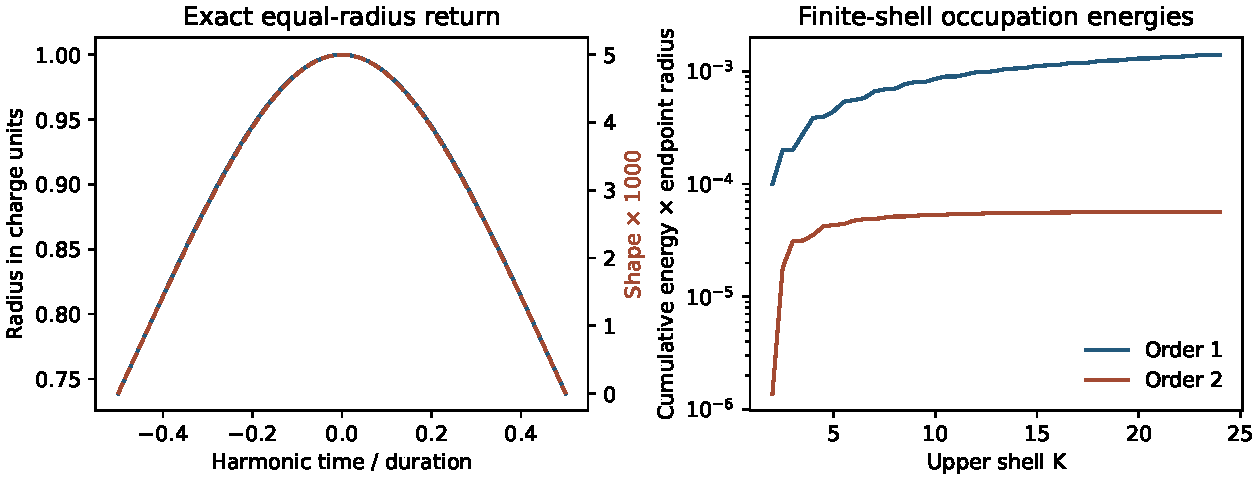
\includegraphics[width=\linewidth]{figures/history.pdf}
\caption{Left: charge-normalized radius (solid) and shape (dashed, right axis) of the exact return. Right: cumulative positive occupation energies through the displayed spherical shells. Each term is obtained from the midpoint of its enclosed probability interval.}\label{fig:history}
\end{figure}
